\chapter{Background}
\section{Related Research}
  \subsection{Problem Definition}
  % TODO: MIKAL transitions and stress.
  % TODO: Shor - support from family lowers mortality

  \subsection{Obstacles}
  % TODO: Flynn - Underestimating Compliance
  % TODO: Lee - tough don't ask for help.

  \subsection{Positive Influences}
  % TODO: Vachon - social support and bereavement
  % TODO: Lehman - fguring out what is useful to bereaved.
  % TODO: HJO - SNS and feelings of support.

\section{Related HCI Work}
  \subsection{Bereavement Technologies}
  Research into bereavement from the perspective of HCI is young, but the
  existing literature reveals some of the core problems that technology can
  address. Among the earliest research is that of Massimi and Baecker in 2010
  \cite{mm10},
  a needs-analysis of all the ways that technology intersects with the lives of
  the bereaved.
  Part of their study was an observation of how,
  in the potentially-dispersed setting of the modern world, 
  technology is already used to help bring people together during mourning.
  Massimi and Baecker proposed a wide set of design opportunities and challenges.
  They were primarily interested in exploring technological artifacts,
  both inherited from the deceased and those created by the bereaved to
  remember and grieve, but they also mention the possibility of technology
  helping to provide social support.

  % Homescreen Figure
  \begin{figure}
  \caption{\textbf{Besupp Screenshot} --
  Besupp offered circles for people with like losses to share thoughts
  and feelings with each other.
  }
  \centering
  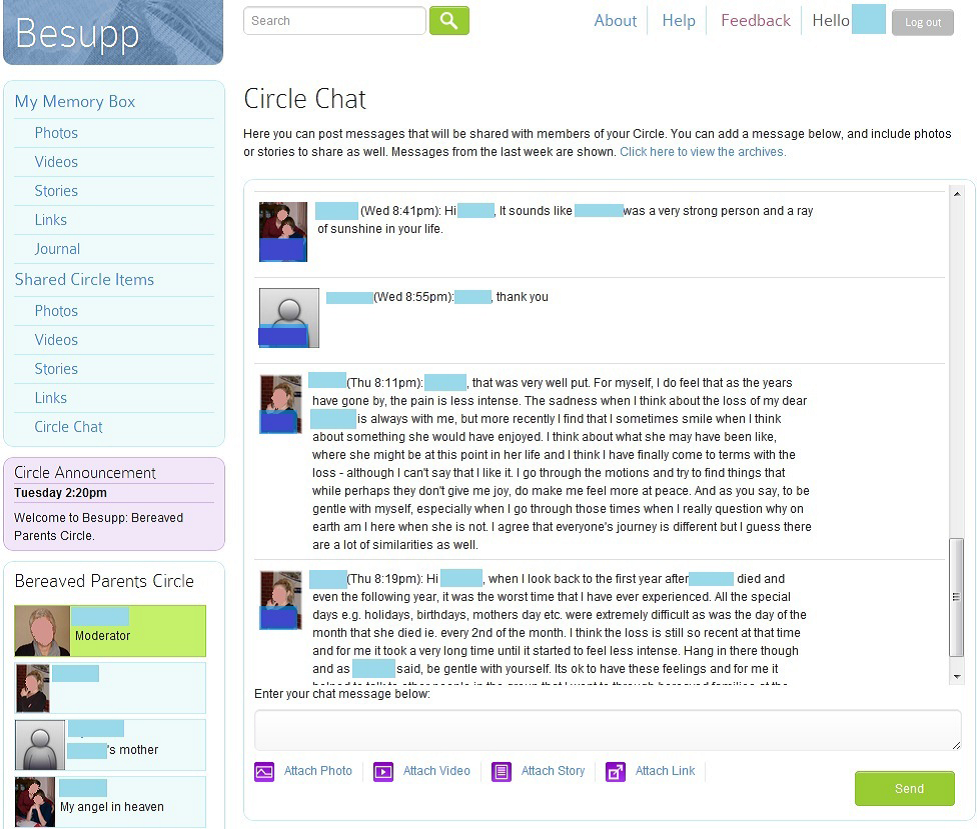
\includegraphics[width=0.65\textwidth]{besupp.png}
  \label{fig:besupp}
  \end{figure}

  There have been few technologies designed explicitly for the grieving. One
  example is Besupp, an online platform for maintaining a support group between
  people who have experienced similar losses, designed and tested by Massimi and
  co. in 2013. \cite{mm13}
  A screenshot from the study is shown in Figure \ref{fig:besupp}.
  Massimi and co. observed that technologies can be helpful as
  one of many ways to help with coping, as the needs of the bereaved are best
  addressed by a variety of interactions.
  This further study demonstrated that
  there is value in support systems that are maintained over long periods and
  designed for to low and intermittent usage.

  Other research has generally been observational, for instance Brubaker's study
  in 2011 of usage of existing technologies. \cite{brubaker11}

  \subsection{Communication Technologies}
  When it comes to the practical aspect of designing for interpersonal
  communication, researchers in family interactions have significant experience.
  Designing technologies for a multi-person group is unusual because the usual
  standards of usability need to be applied to the unit as a whole, and not just
  the experience of a particular individual. \cite{neustaedter12}

  I am interested in technologies classified as "interpersonal awareness systems,"
  designed to be used by families and couples that are separated by distance.
  Systems like this help people maintain awareness of  of each other to connect
  and comfort each other. \cite{neustaedter06}
  In 2004, Markopoulos designed and tested an
  awareness system for families that shared pictures and snippets from a mobile
  device, demonstrating the value of mediating that connection through technology.
  \cite{markopoulos04}
  My theory is that the support of intimate family relations is a powerful
  resource that could
  have a very positive influence on the experience of bereaved individuals.

  %TODO SKEELS - breast cancer help.
  %TODO Granholm - MATS, schizophrenia

\section{Technology and Stress}





